
%----------------------------------------------------------------------------------------
%	CHAPTER 4  MIRT Eye Tracking Algorithm
%----------------------------------------------------------------------------------------
\chapterimage{eyes_women_cropped.jpg}
\chapter{MIRT} \index{MIRT}
\label{ch_mirt}
In this chapter we present MIRT: Morphological Based Iris Tracking a novel method for real-time iris detection and tracking. MIRT is a morphological based real-time iris detection algorithm. Morphological operations are simple and fast to compute which reduces the time required to detect the iris. 

Two typed of image processing in eye tracking are used; visible and infrared spectrum imaging. Most available eye tracking approaches like Starburst \cite{starburst} and Pupil \cite{pupil} rely on infrared spectrum imaging. It's known that visible spectrum imaging is more complicated due to the uncontrolled ambient light that is used as a light source which usually contains multiple specular and diffuse components. On the other hand infrared imaging eliminates uncontrolled specular reflection by illuminating the eye with a uniform and controlled infrared light \cite{starburst}. However, infrared imaging requires using special hardware (infrared cameras, infrared lights). MIRT uses visible imaging to track the iris. Not to mention that MIRT can be used outdoors which is not available using infrared based eye-tracking algorithms We also doesn't require any special hardware, we use a low resolution web-cam. Used hardware and head-mounted tracker will be discussed later in this book.\bigskip


\section{Overview}\index{Overview}
MIRT algorithm can be divided into 2 stages; 1) locating region of interest in the given image, and 2) detecting the iris in the region of interest located in stage 1. At first we transform the input frame to gray scale then we locate the parts of the visible parts of the sclera. Next we estimate the location of the iris based on the location of the sclera, and we crop the region of interest (ROI) from the source image. We try to minimize the ROI as possible to cut down the runtime and to minimize the error of the estimated iris center. From the extracted ROI we find the a set of feature points. An inlier feature points is a point that lies on the edge of the iris. Extracted feature points may contain some outliers, therefore we use RANSAC ellipse fitting to fit ellipse model on the extracted feature points. RANSAC is an effective technique for model fitting in the presence of a large but unknown percentage of outliers in a measurement sample. Using the RANSAC technique increase the ability of the system to do robust estimation of the model (ellipse) parameters. Figure \ref{fig:mirt_overview} shows the stages of the MIRT algorithm.

\begin{figure*}[!h]
\begin{dBox}
\centering
	\mbox{
		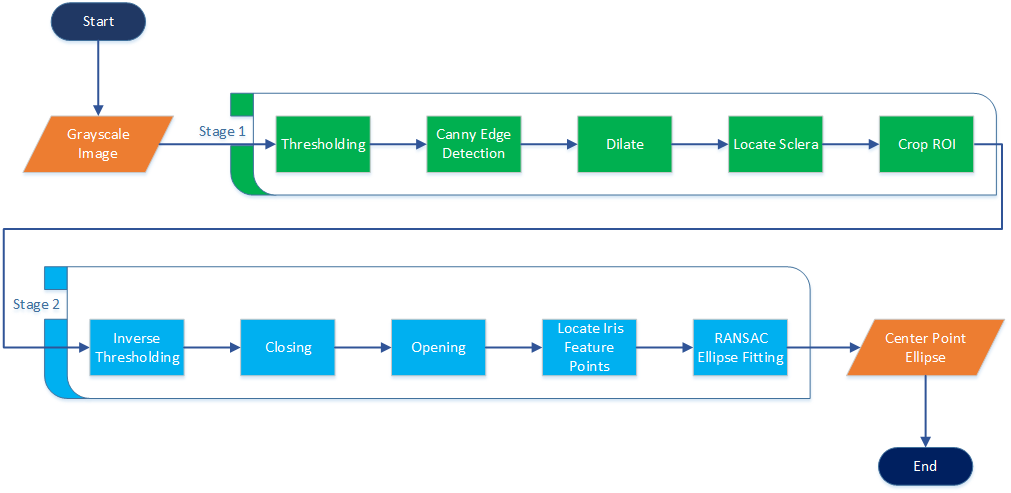
\includegraphics[width=\textwidth]{./Pictures/mirt/MIRT_overview.png}
	}
   \caption{Overview of MIRT Algorithm \label{fig:mirt_overview} }   
\end{dBox}   
\end{figure*}


\section{ROI Localization}\index{ROI Localization}
As figure \ref{fig:mirt_overview} illustrates the pipeline of the ROI localization step. We use simple thresholding on the input gray scale image (frame). Then we apply Canny edge detection algorithm \cite{canny} on the binary image. Then we dilate using a small structuring element just to fill the small gaps between edges and make edges wider. This goal from the dilation step is to increase the robustness of contour finding step. We use circular shaped small structuring element with diameter $ d = 3 $ pixels. \bigskip

The next stage is that we find the largest 2 contours that satisfy the size constrain. We defined a size threshold to eliminate the regions that might be mistaken with the sclera. When the iris is in the middle of limbus (corneal limbus is the border of the cornea and the sclera) 2 parts of the sclera are visible as illustrated in figure \ref{fig:roi_2p}. In this case the largest 2 contours will be two parts of the sclera and the iris is estimated to lie between those two parts. The ROI is set to be the bounding box of the two contours, shown in figure \ref{fig:roi_2p}. \bigskip

\begin{figure*}[!h]
\begin{dBox}
	\mbox{
	\centering
		\subfigure[Input image]{
			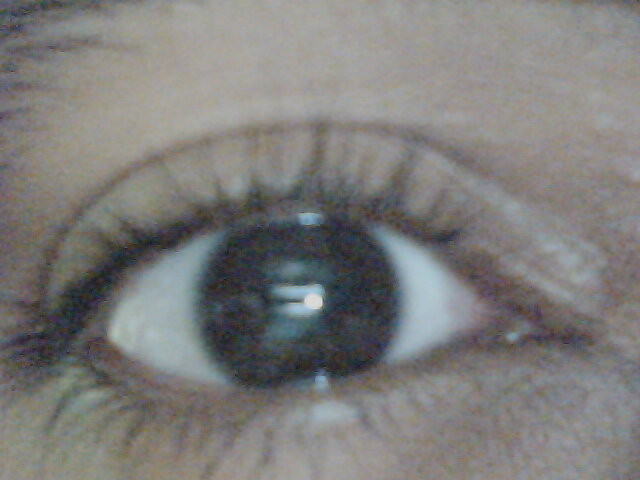
\includegraphics[width=.31\textwidth]{./Pictures/mirt/3.jpg}
			\label{fig:input_2p}
        }
        \subfigure[Illustration of stage 1]{
			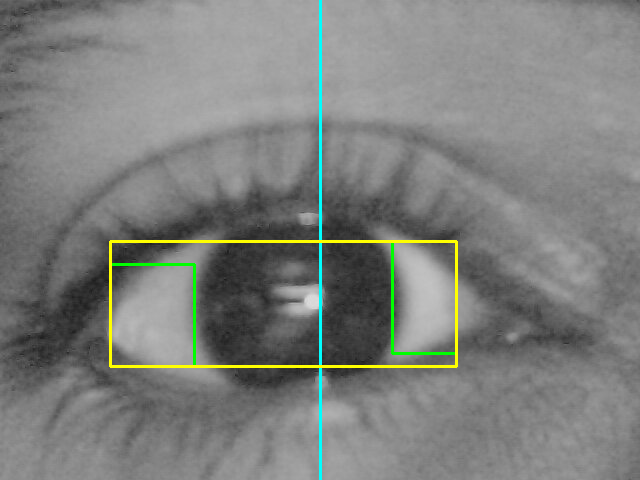
\includegraphics[width=.31\textwidth]{./Pictures/mirt/locate_roi_2p.png}
			\label{fig:roi_2p}
        }
        \subfigure[Algorithm output]{
			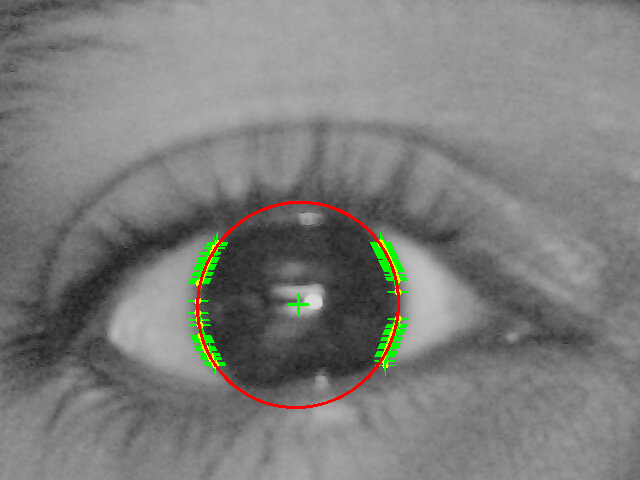
\includegraphics[width=.31\textwidth]{./Pictures/mirt/result_2p.png}
			\label{fig:result_2p}
        }
	}
   \caption{MIRT in action when 2 parts of sclera are visible; (a) shows the input image. (b) shows the 2 parts of sclera marked with green, ROI marked with yellow, and previous estimation of pupil center x with cyan. (c) shows the estimated ellipse with red and feature points with green cross-hairs. \label{fig:mirt_2p} }      
\end{dBox}   
\end{figure*}



\begin{figure*}[!h]
\begin{dBox}
	\mbox{
		
		\centering
		\subfigure[Input image]{
			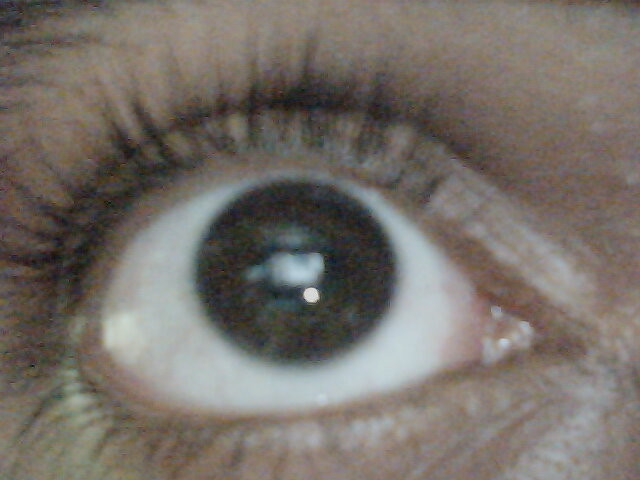
\includegraphics[width=.31\textwidth]{./Pictures/mirt/4.jpg}
			\label{fig:input_1p}
        }
        \subfigure[Illustration of stage 1]{
			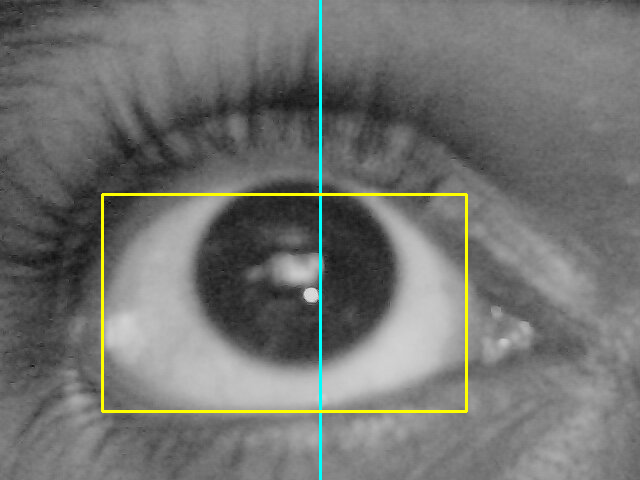
\includegraphics[width=.31\textwidth]{./Pictures/mirt/locate_roi_1p.png}
			\label{fig:roi_1p}
        }
        \subfigure[Algorithm output]{
			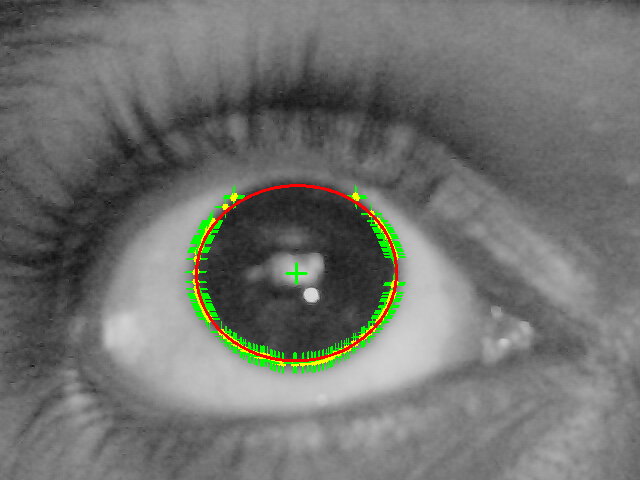
\includegraphics[width=.31\textwidth]{./Pictures/mirt/result_1p.png}
			\label{fig:res_1p}
        } 
    }
\caption{MIRT in action when 2 connected parts of sclera are visible; (a) shows the input image. (b) shows the visible contour of sclera marked with green, ROI marked with yellow, and previous estimation of pupil center x with cyan. (c) shows the estimated ellipse with red and feature points with green cross-hairs. \label{fig:mirt_1p} }      
\end{dBox}
\end{figure*}

In other cases when the iris is either on the left or on the right of the limbus, only one part of the sclera is visible which is the largest contour found in the image, hence we have 3 different situations. If the width of the largest contour is greater than twice the estimated iris size $ h = 150 $ (based on our head mounted camera) then the ROI is the bounding rectangle of the largest contour as illustrated in figure \ref{fig:mirt_1p}. We assume that the iris is nearly at the center of the limbus, yet one of the visible sclera contours couldn't be extracted. \bigskip

% TODO ensure this part is on the same page
For the two other cases we define a placement ratio 
	\begin{dBox}
		\centering
		$$ r = abs ( \frac{ c - x_{start}}{x_{end} - c } ) $$
	\end{dBox}
where $c$ is the x coordinate value of the iris center estimated in the previous frame, $c$ is set to the center of the image in the first frame. $x_{start}$ and $x_{end}$ are the x coordinates of the start and the end of largest contour. In other words $r$ is the ratio between the both sides of the largest contours to the initial center of the pupil. If $r \leq 1 $ then the iris is on the right and the left part of the sclera is visible. The ROI width stretches from $x_{end} - h/2$ to $x_{end} + h $ and have the same hight of the largest. See figure \ref{fig:mirt_l} for illustration. \bigskip

\begin{figure*}[!h]
\begin{dBox}
	\mbox{

        \subfigure[Input image]{
			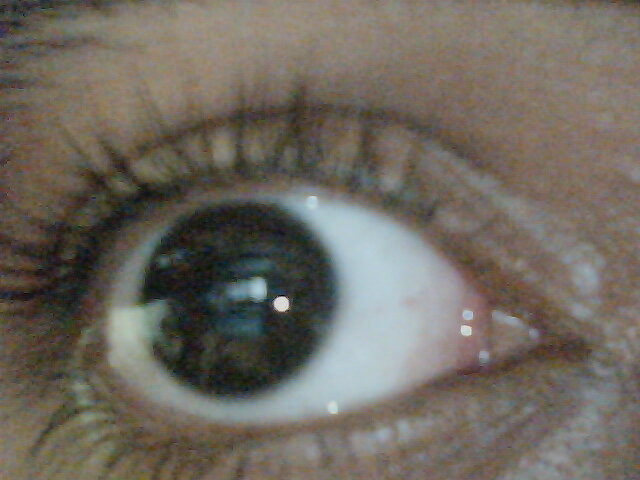
\includegraphics[width=.31\textwidth]{./Pictures/mirt/2.jpg}
			\label{fig:input_l}
        }
        \subfigure[Illustration of stage 1]{
			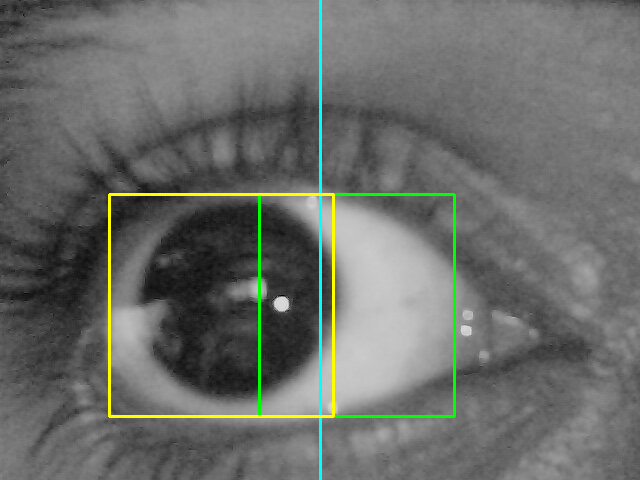
\includegraphics[width=.31\textwidth]{./Pictures/mirt/locate_roi_l.png}
			\label{fig:roi_l}
        }
        \subfigure[Algorithm output]{
			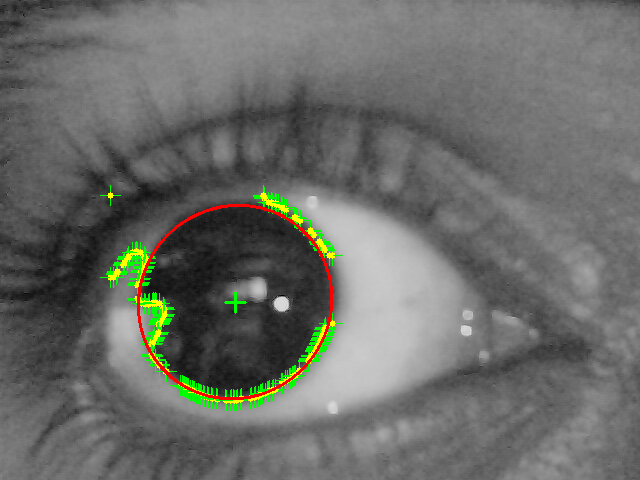
\includegraphics[width=.31\textwidth]{./Pictures/mirt/result_l.png}
			\label{fig:res_l}
        } 
    }|    
\caption{MIRT in action when the right side of sclera is visible; (a) shows the input image. (b) shows the visible (right) side of sclera marked with green, ROI marked with yellow, and previous estimation of pupil center x with cyan. (c) shows the estimated ellipse with red and feature points with green cross-hairs. \label{fig:mirt_l} }      
\end{dBox}
\end{figure*}

The opposite case is that if $r > 1$ then the iris is in the left and the right part of the sclera is visible. Similar to the previous case the ROI is set to be $x_{start} - h$ to $x_{start} + h/2 $ in width and also have the same height of the largest contour. Figure \ref{fig:mirt_r} shows this case. One last case remaining is that none of the found contours satisfied the size condition, this situation can occur in frames where the limbus is not visible (i.e blink), hence the frame is skipped. Finally if the estimated bounds of the ROI are outside input image boundaries the ROI boundaries are clamped to the input image bounds. Algorithm \ref{mirt_roi_loc_algo} illustrates the procedure of MIRT ROI localization stage.

\begin{figure*}[!h]
\begin{dBox}
	\mbox{

        \subfigure[Input image]{
			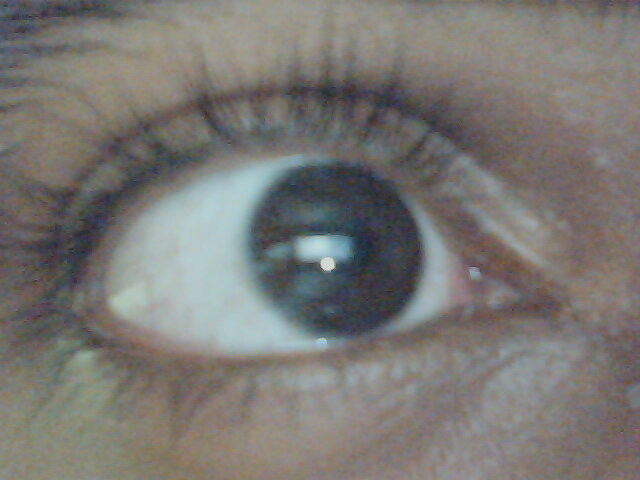
\includegraphics[width=.31\textwidth]{./Pictures/mirt/1.jpg}
			\label{fig:input_r}
        }
        \subfigure[Illustration of stage 1]{
			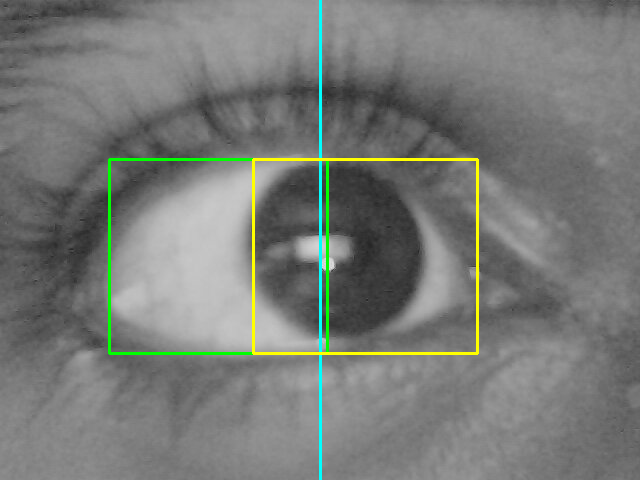
\includegraphics[width=.31\textwidth]{./Pictures/mirt/locate_roi_r.png}
			\label{fig:roi_r}
        }
        \subfigure[Algorithm output]{
			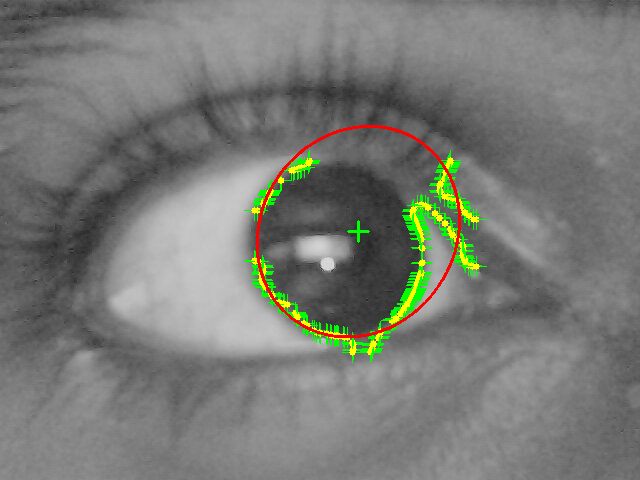
\includegraphics[width=.31\textwidth]{./Pictures/mirt/result_r.png}
			\label{fig:res_r}
        } 
	}

\caption{MIRT in action when the left side of sclera is visible; (a) shows the input image. (b) shows the visible (left) side of sclera marked with green, ROI marked with yellow, and previous estimation of pupil center x with cyan. (c) shows the estimated ellipse with red and feature points with green cross-hairs. \label{fig:mirt_r} }      
\end{dBox}
\end{figure*}

\begin{algorithm}[!h]
\begin{dBox}

	\caption{MIRT: Locate ROI (Stage 1)} \label{mirt_roi_loc_algo}
	\begin{algorithmic}[1]
		\Require{grayscale eye image}
		\Ensure {grayscale ROI image}
		\Procedure{MIRT: locate ROI}{}
		\State $binary \gets$ \Call{threshold}{$input$}
		\State $edges \gets$ \Call{canny}{$binary$}
		\State \Call{dilate}{$edges$}
		\State $largest,\: secondlargest \gets$ \Call{findContours}{$edges$}

		\If{\Call{area}{largest} < $AREA\_THRES$} \Comment{no valid contours found}
			\State terminate
		\ElsIf{\Call{area}{$secondlargest$} < $AREA\_THRES$}  \Comment{only 1 contour found}
			\State $c \gets previous\_center.x$
			\State $r \gets (c-x_{start})/(x_{end}-c)$

			\If{$largest.width > 2*IRIS\_SIZE$}
				\State $ROI \gets$ \Call{rectangle}{$largest$}
			\ElsIf{$r < 1$}	\Comment{right part visible}
				\State $ROI.x_{start} \gets largest.x_{start} - IRIS\_SIZE $
				\State $ROI.x_{end} \gets largest.x_{start} + IRIS\_SIZE/2$
			\Else  \Comment{left part visible}
				\State $ROI.x_{start} \gets largest.x_{end} - IRIS\_SIZE/2 $
				\State $ROI.x_{start} \gets largest.x_{end} + IRIS\_SIZE$
			\EndIf

		\Else  
			\Comment{2 contour found}
			\State $ROI \gets $\Call{boundingrectangle}{$largest, \: secondlargest$}
		\EndIf

		\Call{crop}{$input, \: ROI$} 
		\Comment{crop the input image to the ROI}
		
		\Return $ROI$
		\EndProcedure	
	\end{algorithmic}
\end{dBox}	
\end{algorithm}



\section{Locate Iris In ROI} \index{Locate Iris In ROI}
In this stage we are interested in finding the iris in the tightly cropped ROI located in stage 1. we start by applying inverse simple thresholding to filter dark areas in the ROI. Next we apply morphological closing followed by opening using 19 pixel circular structuring element. The main goal of this step to fill the gaps in the iris (gaps come from light reflections) and to open between the iris and other parts of the ROI that passed through the thresholding step. Then we find the largest contour in the ROI. In almost all cases the largest contour will contain the iris as shown in figure \ref{fig:iris_contour}. Finally we extract feature points from the largest contour. Edge points of the contour are considered as feature points. We use Random Sample Consensus (RANSAC) paradigm for model fitting \cite{ransac}. RANSAC is an effective technique for model fitting in the presence of a large but unknown percentage of outliers in a measurement sample. In our application inliers are feature points that lie on the iris contour, while outliers are feature points that belong to other contours other than the iris contour. Using the RANSAC technique increase the ability of the system to do robust estimation of the model (ellipse) parameters. We draw 5 samples from the detected feature set, then we compute the best fit ellipse using Fitzgibbon’s algorithm \cite{fitzgibbon96} which is implemented in OpenCV. Finally we evaluate the error between the estimated model and all feature points and count inliers / outliers. Algorithms \ref{mirt_iris_algo} and \ref{our_ransac} summarizes stage 2 procedure and how we use RANSAC in our system respectively. Figure \ref{fig:loc_iris} shows the steps of stage 2. 


\begin{figure}[!h]
\begin{dBox}
	
	\centering
	\mbox{
        \subfigure[Grayscale ROI]{
			
\includegraphics[width=.49\textwidth]{./Pictures/mirt/ROI.png}
			\label{fig:iris_roi}
        }

		\subfigure[Binary]{
			
\includegraphics[width=.49\textwidth]{./Pictures/mirt/binary.png}
			\label{fig:iris_binary}
        } 
    } 
    \mbox{
        \subfigure[Closing/Opening]{
			
\includegraphics[width=.49\textwidth]{./Pictures/mirt/morph.png}
			\label{fig:morph}
        }
        \subfigure[Largest Contour / Feature Points]{
			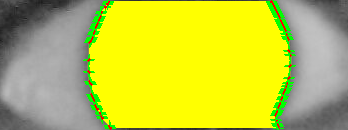
\includegraphics[width=.49\textwidth]{./Pictures/mirt/contour.png}
			\label{fig:iris_contour}
        } 
    }    
    \mbox{    
         \subfigure[Estimated Ellipse]{
			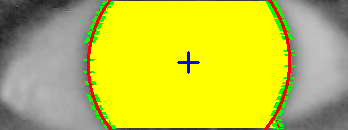
\includegraphics[width=.49\textwidth]{./Pictures/mirt/color_roi.png}
			\label{fig:iris_ellipse}
        } 
	}

\caption{Visualization of MIRT stage 2. (a) shows the input cropped ROI, (b) shows the binary image after inverse thresholding, (c) shows the binary image after performing closing followed by opening, (d) visualizes the largest contour in the image (colored with yellow) and extracted feature points marked with green cross-hairs and red points, (e) shows the estimated ellipse with red curve. \label{fig:loc_iris} }      
\end{dBox}
\end{figure}



\begin{algorithm}[!h]
\begin{dBox}
	\caption{MIRT: Locate Iris (Stage 2)} \label{mirt_iris_algo}
	\begin{algorithmic}[1]
		\Require{grayscale ROI image}
		\Ensure {Ellipse that describes the iris}
		\Procedure{MIRT: locate Iris}{}
		\State $binary \gets$ \Call{inversethreshold}{$input$}
		\State \Call{closing}{$binary$}
		\State \Call{opening}{$binary$}
		\State $largestcontour \gets$ \Call{findContours}{$binary$}
		\State $ellipse \gets$ \Call{RANSAC\_ellipse\_fitting}{$largestcontour$}
		\State \Return $ellipse$
		\EndProcedure	
	\end{algorithmic}
\end{dBox}	
\end{algorithm}


\begin{algorithm}
\begin{dBox}
	\caption{Our RANSAC Ellipse Fitting Procedure} \label{our_ransac}
	\begin{algorithmic}[1]
		\Procedure{RANSAC\_ellipse\_fitting}{}
		 \While{$i < N$}
			\State Draw $s$ points uniformly at random
			\State Fit ellipse model to these $s$ points
			\State Find inliers to this ellipse (points whose algebraic error $ < t$)
			\State If there are $d$ or more inliers, accept the ellipse and refit using all inliers	
		\EndWhile	
		\EndProcedure	
	\end{algorithmic}
\end{dBox}	
\end{algorithm}
